
\documentclass[12pt]{article}
\usepackage{amsmath}
\usepackage{amsfonts}
\usepackage{amssymb}
\usepackage{geometry}
\usepackage{graphicx}
\geometry{a4paper, margin=0.8in}
\pagenumbering{gobble}

\title{Homework assignment for 02YELMA \\ Chapter: Electrodynamics}
\begin{document}
\date{}
\maketitle
\vspace{-0.8in}

\begin{enumerate}

    \item 
    \begin{figure}[htbp]
    \centering
    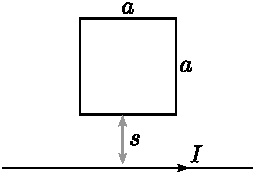
\includegraphics[width=0.3\textwidth]{q1.pdf}
    \end{figure}
    A square wire loop lies a distance $s$ from a very long straight wire that holds a current $I$ as shown above. Find the flux of magnetic field $\Phi$ through the loop. If the wire is pulled directly away from the wire at speed $v$ what emf is generated and in what direction does the current flow?

    \item A long solenoid of radius $a$ is driven by an alternating current so that the field inside is sinusoidal: $\vec{B}(t)=B_0\cos{\left(\omega t\right)}\hat{z}$. A circular loop of wire of radius $a/2$ and resistance $R$ is placed inside the solenoid and coaxial with it. Find the current induced in the look as a function of time.
    \item Find the self-inductance per unit length of a long solenoid, of radius $R$, carrying $n$ turns per unit length.

    \item Find the self-inductance per unit length of a long solenoid of radius $R$ with $n$ turns per unit length.
    \item A \emph{sufficiently long} solenoid with radius $a$ and $n$ turns per unit length carries a time-dependent current $I(t)$ in the $\hat{\phi}$ direction. Find the electric field (direction and magnitude) at a distance $s$ from the axis of the solenoid (both inside and outside the solenoid) in the \emph{quasi-static approximation}.
    \begin{itemize}
        \item \emph{Sufficiently long}: There is a uniform magnetic field inside the solenoid and negligible field outside.
        \item \emph{Quasi-static approximation}: The change in the magnetic field is slow enough that the rules of magnetostatics apply to determine the magnetic field at a given time.
    \end{itemize}
    \item A parallel-plate capacitor of plate radius $R$ and plate separation $d$ is being driven by a sinusoidal voltage $V(t)=V_0\cos (\omega t)$ across its plates. The space between the plates is vacuum. 
    \begin{itemize}
        \item[(a)] Compute the displacement current $\vec{J}_d(t)$ flowing between the plates.
        \item[(b)] Compute the magnitude of magnetic field $B(r,t)$ at a distance from the capacitor axis. 
    \end{itemize}

\end{enumerate}



\end{document}
